%Rendering of the simplest possible Graph
\begin{figure}
    \begin{center}
        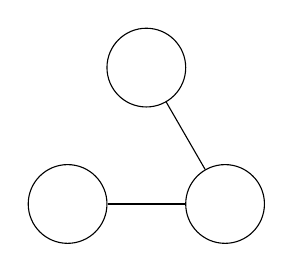
\begin{tikzpicture}
            % Define vertices
            \node[circle,draw,minimum size=1cm] (A) at (0,0) {};
            \node[circle,draw,minimum size=1cm] (B) at (2,0) {};
            \node[circle,draw,minimum size=1cm] (C) at (1,1.732) {};
            
            % Draw edges
            \draw (A) -- (B);
            \draw (B) -- (C);
            \end{tikzpicture}
        \caption{A simple graph with three vertices and two edges.}
        \label{Figure:graph-simple}          
    \end{center}
\end{figure}